\documentclass[10pt,a4paper]{article} % tamaño de letra y tipo de papel
\usepackage[utf8]{inputenc}
\usepackage[spanish]{babel} % paquete para que reconozca ñ y tildes
\usepackage{amsmath}
\usepackage{amsfonts}
\usepackage{amssymb}
\usepackage{graphicx} % paquete para incluir imagenes
\usepackage[margin=1in,bottom=1in]{geometry}
\usepackage{hyperref} % paquete para tener marcadores en el pdf
\author{Ulloa Daniel}
\begin{document}

\begin{titlepage}
	\hbox{
		\hspace*{0.15\textwidth} % Espacio desde el margen izquierdo
		\rule{1pt}{\textheight} % Linea decorativa
		\hspace*{0.05\textwidth} % Espacio entre la linea y el texto
		\parbox[b]{0.75\textwidth}{ % Caja que restringe el espacio que puede ocupar el texto
			{\noindent\Huge\bfseries Informe de Laboratorio } % Titulo
			\\ 
			[2\baselineskip] 
			{\large \textbf{Tema:} Oscilador con Resistencia Negativa} % Tema
			\\[4\baselineskip]
            {\large \textbf{Cátedra:} Teoría de Circuitos \textsc{II}} % Catedra
            \\[1\baselineskip]
            {\large \textbf{Año:} 2019} % Año
			\\[1\baselineskip]
            {\large \textit{\textbf{Docentes:} % Docentes
                \textnormal{Ing. Costa}, Nicolás. 
                \textnormal{Aux. Consiglio}, Dante}
            }
			\\[1\baselineskip]
            {\large \textit{\textbf{Alumnos:} % Alumnos
                \textnormal{Rodriguez}, Ana Victoria. 
                \textnormal{Ulloa}, Daniel Alejandro}
            }
            \\[6\baselineskip]
            {\large \textbf{Fecha de Entrega:} 11/09/2019}
			\par %Para que el logo aparezca al pie
			\vspace{0.35\textheight} % Ubicacion de la caja desde el margen superior
            \center{
\includegraphics[width=250px]{logo2.png}}
            \\[1\baselineskip]
	}}
\end{titlepage}
\tableofcontents
\newpage
\section{Introducción}

\section{Objetivos}
\begin{itemize}
    \item Modelar e interpretar el Circuito
    \item Obtener la respuesta temporal de la tensión de salida y graficarla en Mathematica
    \item Realizar un barrido paramétrico sobre la resistencia $R_B$ y observar las diferentes respuestas.
\end{itemize}
\section{Modelado Matemático}
El circuito a modelar se muestra a continuación %sopenca
\begin{center}
    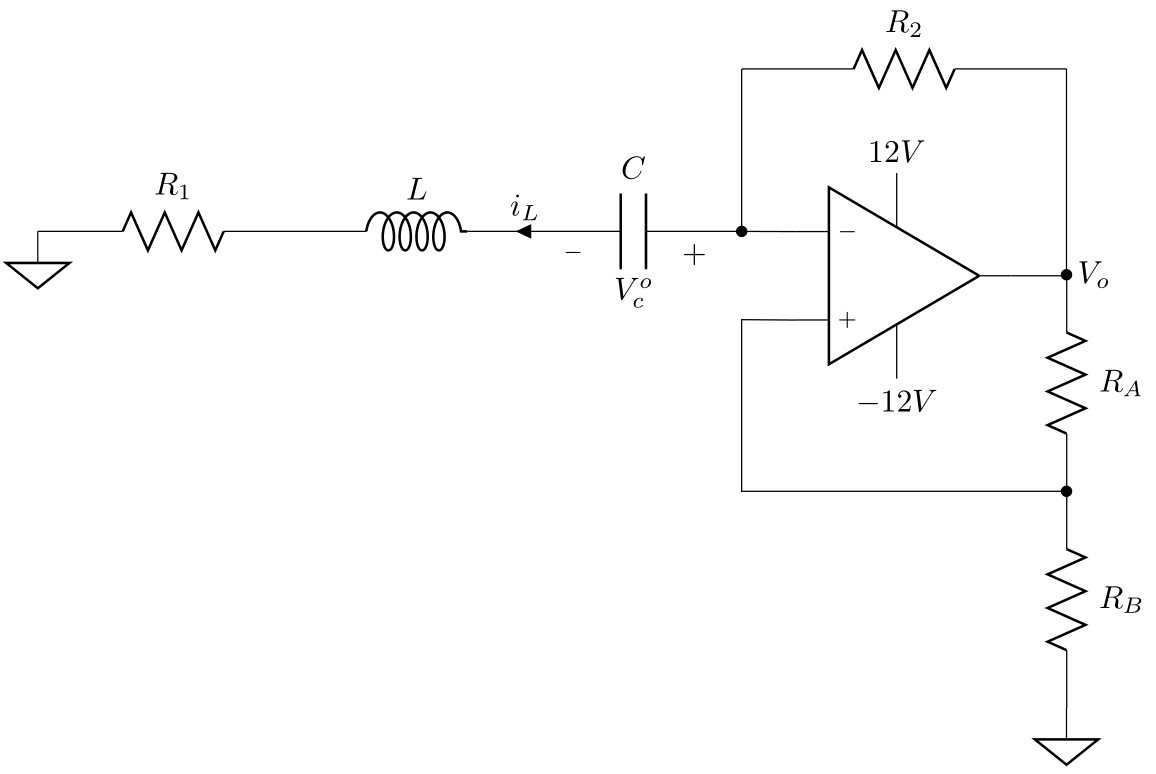
\includegraphics[width=300px]{circuito}
\end{center} 
%Agrego cada equacion que deje en comentarios en mathematica o solo las que utilizamos? 
Para la primera ecuación se analizó el nodo Vn y se considero que el amplificador operacional es ideal, entonces $i_{n}[t]=0$
y la corriente que pasa por %la rama RLC (il) es igual a la corriente que pasa por la resistencia R2.
%\text{il}=\text{C1} \text{Vc}'(t);i \text{R2}=\frac{\text{Vn}-\text{Vo}(t)}{\text{R2}};\text{Vn}=\frac{\text{RB} \text{Vo}(t)}{\text{RA}+\text{RB}};i \text{R2}=\frac{(-\text{Ra}) \text{Vo}(t)}{\text{R2} (\text{Ra}+\text{Rb})};\frac{(-\text{Ra}) \text{Vo}(t)}{\text{R2} (\text{Ra}+\text{Rb})}=\text{C1} \text{Vc}'(t)

 \begin{equation}
\text{eq1}=\text{C1} s \text{Vc}(s)-\text{C1} \text{v0}(t)+\frac{\text{Ra} \text{Vo}(s)}{\text{R2} (\text{Ra}+\text{Rb})}=0
\end{equation}

\begin{equation}
\text{eq2}=\text{C1} \text{L1} \left(s^2 \text{Vc}(s)-s \text{v0}(t)\right)+\text{C1} (\text{R1}+\text{R2}) (s \text{Vc}(s)-\text{v0}(t))+\text{Vc}(s)-\text{Vo}(s)=0
\end{equation}




\section{Respuesta Temporal}
\section{Barrido Paramétrico}
\section{Conclusión}
\end{document} 

%el tema es como haces vos para ver el pdf que se va generando ?

